\documentclass[final,t]{beamer}
\mode<presentation>{ \usetheme{Major} }
\usepackage{times}
\usepackage{amsmath,amsthm, amssymb, latexsym}
\boldmath
\usepackage[english]{babel}
\usepackage{relsize}
\usepackage{multirow}
%\usepackage{qtree}
\usepackage{stmaryrd}
\usepackage{booktabs}

%  \usepackage[font=small,format=plain,labelfont=bf,up,textfont=it,up]{caption}
\usepackage[font=normalsize,labelfont=small,bf,margin=2cm]{caption}
\usepackage[latin1]{inputenc}
\usepackage[orientation=portrait,size=a0,scale=1.4,debug]{beamerposter}
\usepackage{color,listings}
\usepackage{calc,xcolor}
\usepackage[absolute,overlay]{textpos}
\usepackage{smartdiagram}
\usepackage{wrapfig}
\usepackage[many]{tcolorbox}
\usepackage{tikz}
\usetikzlibrary{shadings}


\long\def\omitit#1{} % used to comment-out /remove text at compile-time.

%\definecolor{lightblue}{rgb}{.85,.85,1} % 217 217 255
%\definecolor{lightorange}{rgb}{1,.8,.6} % 255 204 153
%\definecolor{lightgreen}{rgb}{.77,.91,.5} % 196 232 128
%\definecolor{lightyellow}{rgb}{1,.98,.6} % 255 250 153
%\definecolor{prussianblue}{rgb}{0.0,0.19,0.33}
%\definecolor{gold}{rgb}{0.6,0.4,0.08}


%\setbeamercolor{caption name}{fg=prussianblue} %''Figure'' titles colour
\setbeamercolor{caption name}{fg=britishRacingGreen} %''Figure'' titles colour

\makeatletter
\pgfdeclarehorizontalshading{beamer@headfade}{5.4375ex+490pt}
{%
  color(0cm)=(lightblue);
  % color(15cm)=(lightblue);
  color(45cm)=(lightyellow);
  color(\paperwidth)=(gold)%
}
\addtoheadtemplate{\pgfuseshading{beamer@headfade}\vskip\dimexpr 0pt-52ex}{}
\makeatother


\newsavebox\CBox
\newenvironment{ColorBox}[3][black]{
    \par\noindent
    \def\borderColor{#1}\def\bgColor{#2}
    \begin{lrbox}{\CBox}
    \minipage{#3-2\fboxsep-2\fboxrule}
}{
    \endminipage\end{lrbox}%
    \fcolorbox{\borderColor}{\bgColor}{\usebox\CBox}\par
}

\lstset{language=java}
\lstset{breaklines=true}
\lstset{showstringspaces=false}
\lstset{tabsize=3}
\lstset{basicstyle=\ttfamily\scriptsize}
\lstset{breakautoindent=true}
\lstset{postbreak=\space}
%\lstset{commentstyle=\color{XcodeComments}}
%\lstset{keywordstyle=\color{XcodeKeywords}}
%\lstset{stringstyle=\color{XcodeStringstyle}}

%%%%%%%%%%%%%%%%%%%%%%%%%%%%%%%%%%%%%%%%%%%%%%%%%%%%%%%%%%%%%%%%%%%%%%%%%%%%%%%%%5
\title[]{Text mining in Python for Evaluating the Ethical Foundations in Computer Science}
\author[Bonham-Carter]{Enpu You, Oliver Bonham-Carter, Janyl Jumadinova}
\institute{Dept of Computer Science, Allegheny College \\ Meadville, PA}
\webpage{https://csethics.allegheny.edu}
\mail{\{youe2, obonhamcarter, jjumadinova\}@allegheny.edu}


%%%%%%%%%%%%%%%%%%%%%%%%%%%%%%%%%%%%%%%%%%%%%%%%%%%%%%%%%%%%%%%%%%%%%%%%%%%%%%%%%
\begin{document}
    \begin{frame}{}
        \vspace*{9mm} % was 2
        \begin{columns}[t]
        	\begin{column}{1\linewidth}
%%%%%%%%%%%%%%%%%%%%%%%%%%%%%%%%%%%%%%%%%%%%%%%%%%%%%%%%%%%%%%%%%%%%%
%
% Center column - Context
%
%%%%%%%%%%%%%%%%%%%%%%%%%%%%%%%%%%%%%%%%%%%%%%%%%%%%%%%%%%%%%%%%%%%%%

%%%%%%%%%%%%%%%%%%%%%%%%%%%%%%%%%%%
%
% Project Objectives
%
%%%%%%%%%%%%%%%%%%%%%%%%%%%%%%%%%%%
                \begin{block}{\textsc{\textbf{Project Objectives}}}
				\vspace*{2.0mm}

		\begin{wrapfigure}{r}{0.25\textwidth}
					\begin{figure}
						\centering
						
\includegraphics[scale = .25]{graphics/MozillaLogo_BW.jpg}
                        \caption{\ref{fig:MozillaLogo_BW}. \small \textbf{This project is supported by the Responsible Computer Science Challenge, funded by Omidyar Network, Mozilla, Schmidt Futures and Craig Newmark Philanthropies.}}
                        \label{fig:MozillaLogo_BW}
					\end{figure}
                        \end{wrapfigure} 

                        We present an automated text-mining tool written in Python to measure the technical responsibility of students in computer science courses.

				\begin{itemize}
					\item Our tool automatically collects reflection documents written by students from their GitHub repositories.
					\item Then, using natural language processing analyzes them for ethical considerations based on pre-determined questions and criteria. 
					\item The tool helps to track the progression of student ethical understanding and sense of social responsibility by analyzing writing samples across the computer science curriculum.

				\end{itemize}

                    \vspace*{6mm}
                \end{block}
			\end{column}
		\end{columns}

%%%%%%%%%%%%%%%%%%%%%%%%%%%%%%%%%%%%%%%%%%%%%%%%%%%%%%%%%%%%%%%%%%%%%

		\begin{columns}

%%%%%%%%%%%%%%%%%%%%%%%%%%%%%%%%%%%%%%%%%%%%%%%%%%%%%%%%%%%%%%%%%%%%%
%
% Left column - Context
%
%%%%%%%%%%%%%%%%%%%%%%%%%%%%%%%%%%%%%%%%%%%%%%%%%%%%%%%%%%%%%%%%%%%%%
            \begin{column}{.5\linewidth}
%%%%%%%%%%%%%%%%%%%%%%%%%%%%%%%%%%%
%
% Method
%
%%%%%%%%%%%%%%%%%%%%%%%%%%%%%%%%%%%
			\begin{block}{\textsc{\textbf{Teaching responsible computing}}}
				\vspace*{3mm}

Teaching responsible computing is critical in developing software that produces a positive impact on our society, economy, and individuals.
				\begin{itemize}
					\item  Each application course in computer science at Allegheny College integrates ethical considerations in its pedagogy.
					\item Broad learning categories include topics of internet health, ethics and responsible computing customized to each application course. 
					\item The delivery of these concepts include readings,  discussions, class and lab assignments with heavy software development emphasis. 
					\item As an output, students  write reflection reports to demonstrate their understanding of relevant issues,  ability to analyze information, and  capacity for integrating the understanding and analysis of ethical thinking into their own work.
				\end{itemize}
				\vspace*{2mm}
			\end{block}
%%%%%%%%%%%%%%%%%%%%%%%%%%%%%%%%%%%
%
% Design
%
%%%%%%%%%%%%%%%%%%%%%%%%%%%%%%%%%%%

  %%%%%


			\begin{block}{\textsc{\textbf{Text Mining Tool to Determine Ethical Pedagogy}}}
			\begin{center}
				\begin{center} \end{center} % drop a line
				\begin{figure}
					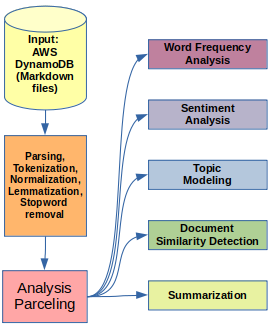
\includegraphics[scale = 3.6]{graphics/flowchart.png}
					\caption{\ref{fig:flowchart}.Simplified Flowchart of tool.}
					\label{fig:flowchart}
				\end{figure}
			\end{center}

				\begin{itemize}
					\item  Our tool first obtains student reflection documents (as Markdown files) stored in AWS.
					\item  Markdown parser goes through the Markdown files and constructs a dictionary.
					\item  Natural language pre-processing is done with SpaCy with the output stored into a pandas data frame for further analysis.
					\item Five categories of analysis are included that can be queried and customized. The result of each analysis is stored in a separate pandas data frame. 
				\end{itemize}
			\vspace*{3mm}
                \end{block}


	\end{column}

%%%%%%%%%%%%%%%%%%%%%%%%%%%%%%%%%%%%%%%%%%%%%%%%%%%%%%%%%%%%%%%%%%%%%
%
% Right column - Outcomes
%
%%%%%%%%%%%%%%%%%%%%%%%%%%%%%%%%%%%%%%%%%%%%%%%%%%%%%%%%%%%%%%%%%%%%%
	\begin{column}{.5\linewidth}
%%%%%%%%%%%%%%%%%%%%%%%%%%%%%%%%%%%
%
%
%
%%%%%%%%%%%%%%%%%%%%%%%%%%%%%%%%%%%


%		\begin{block}{\textsc{\textbf{Features: Word Frequency Analysis}}}
		\begin{block}{\textsc{\textbf{Features}}}
			\vspace*{3mm}

			\begin{figure}
				\begin{tabular}{cc}
					\hspace*{5mm}
					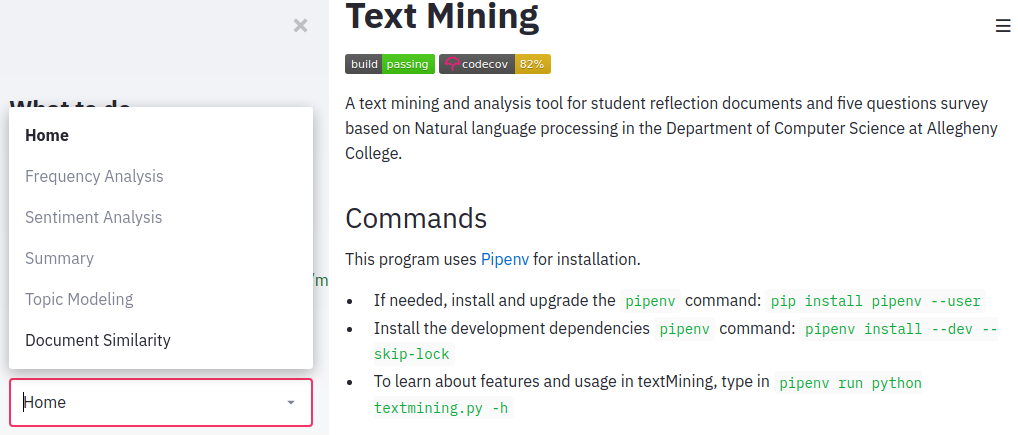
\includegraphics[scale = 1.1]{graphics/interface.png}
				\end{tabular}				
				\caption{\ref{fig:interface} \textbf{Visual Interface}}
				\label{fig:interface}
			\end{figure}

				\begin{itemize}
					\item  Our tool can be run through a command-line  or a graphical interface.
					\item  Visualization was developed using Altair, with the generated graphs displayed using Streamlit.
				\end{itemize}


			\vspace*{3mm}
		\end{block}

                %%%%%%%%%%%%%%%%%%%%%%%%%%%%%%%%%%%
                %
                % Sensors
                %
                %%%%%%%%%%%%%%%%%%%%%%%%%%%%%%%%%%%
		\begin{block}{\textsc{\textbf{Sample Results}}}
			\vspace*{3mm}
			
			\begin{figure}
				\begin{tabular}{cc}
					\hspace*{5mm}
					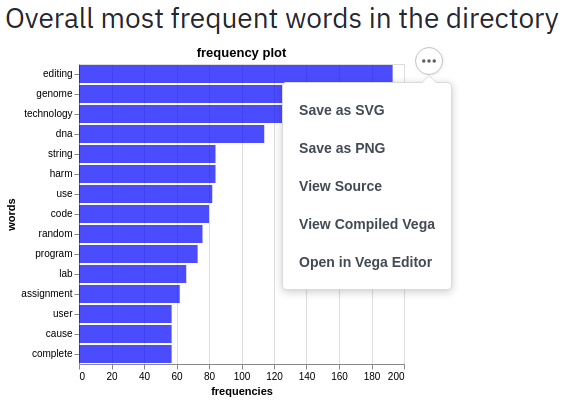
\includegraphics[scale = 1.5]{graphics/freqWords.png}
				\end{tabular}				
				\caption{\ref{fig:freqWords} \textbf{Word Frequency Analysis}}
				\label{fig:freqWords}
			\end{figure}
%			\begin{itemize}
%				\item  bla bla bla
%				\item  bla bla bla
%				\item  bla bla bla
%			\end{itemize}
			\vspace*{3mm}


%		\begin{block}{\textsc{\textbf{Features: Document Similarity}}}
			\vspace*{3mm}
			\begin{figure}
				\begin{tabular}{cc}
					\hspace*{5mm}

					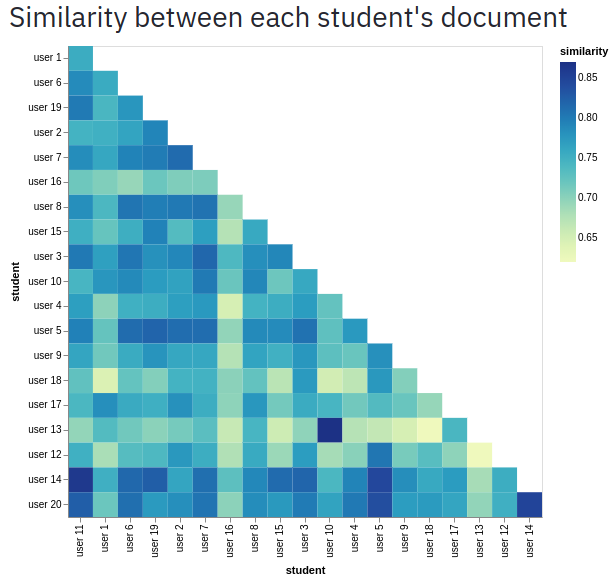
\includegraphics[scale = 1.2]{graphics/docSim.png}
				\end{tabular}				
				\caption{\ref{fig:docSim} \textbf{Document Similarity}}
				\label{fig:docSim}
			\end{figure}
			\vspace*{3mm}
	
%\textbf{This project is supported by the Responsible Computer Science Challenge, funded by Omidyar Network, Mozilla, Schmidt Futures and Craig Newmark Philanthropies.}
	\end{block}

	\end{column}


	\end{columns}
	\end{frame}
\end{document}









%%%%%%%%%%%%%%%%%%%%%%%%%%%%%%%%%%%%
% Junk bin
% Do not delete the following code, but remove it from the project
%%%%%%%%%%%%%%%%%%%%%%%%%%%%%%%%%%%%



